% Graphic for TeX using PGF
% Title: /home/budnyjj/univer/GIT/diploma/b/design/diagrams/ui_hierarchy.dia
% Creator: Dia v0.97.3
% CreationDate: Sun May  8 01:01:27 2016
% For: budnyjj
% \usepackage{tikz}
% The following commands are not supported in PSTricks at present
% We define them conditionally, so when they are implemented,
% this pgf file will use them.
\ifx\du\undefined
  \newlength{\du}
\fi
\setlength{\du}{15\unitlength}
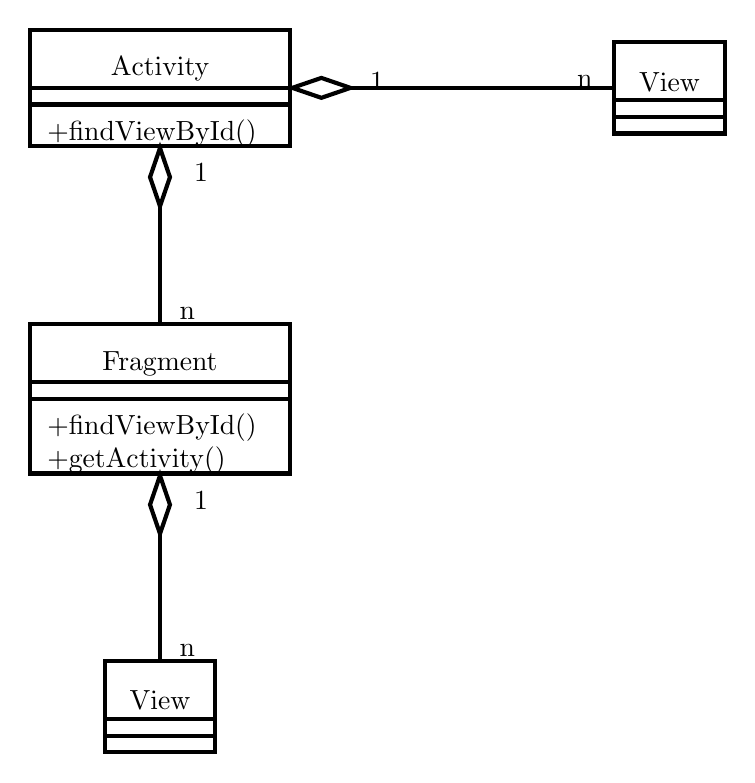
\begin{tikzpicture}
\pgftransformxscale{1.000000}
\pgftransformyscale{-1.000000}
\definecolor{dialinecolor}{rgb}{0.000000, 0.000000, 0.000000}
\pgfsetstrokecolor{dialinecolor}
\definecolor{dialinecolor}{rgb}{1.000000, 1.000000, 1.000000}
\pgfsetfillcolor{dialinecolor}
\pgfsetlinewidth{0.100000\du}
\pgfsetdash{}{0pt}
\definecolor{dialinecolor}{rgb}{1.000000, 1.000000, 1.000000}
\pgfsetfillcolor{dialinecolor}
\fill (6.399601\du,9.226093\du)--(6.399601\du,10.626093\du)--(12.674601\du,10.626093\du)--(12.674601\du,9.226093\du)--cycle;
\definecolor{dialinecolor}{rgb}{0.000000, 0.000000, 0.000000}
\pgfsetstrokecolor{dialinecolor}
\draw (6.399601\du,9.226093\du)--(6.399601\du,10.626093\du)--(12.674601\du,10.626093\du)--(12.674601\du,9.226093\du)--cycle;
% setfont left to latex
\definecolor{dialinecolor}{rgb}{0.000000, 0.000000, 0.000000}
\pgfsetstrokecolor{dialinecolor}
\node at (9.537101\du,10.176093\du){Activity};
\definecolor{dialinecolor}{rgb}{1.000000, 1.000000, 1.000000}
\pgfsetfillcolor{dialinecolor}
\fill (6.399601\du,10.626093\du)--(6.399601\du,11.026093\du)--(12.674601\du,11.026093\du)--(12.674601\du,10.626093\du)--cycle;
\definecolor{dialinecolor}{rgb}{0.000000, 0.000000, 0.000000}
\pgfsetstrokecolor{dialinecolor}
\draw (6.399601\du,10.626093\du)--(6.399601\du,11.026093\du)--(12.674601\du,11.026093\du)--(12.674601\du,10.626093\du)--cycle;
\definecolor{dialinecolor}{rgb}{1.000000, 1.000000, 1.000000}
\pgfsetfillcolor{dialinecolor}
\fill (6.399601\du,11.026093\du)--(6.399601\du,12.026093\du)--(12.674601\du,12.026093\du)--(12.674601\du,11.026093\du)--cycle;
\definecolor{dialinecolor}{rgb}{0.000000, 0.000000, 0.000000}
\pgfsetstrokecolor{dialinecolor}
\draw (6.399601\du,11.026093\du)--(6.399601\du,12.026093\du)--(12.674601\du,12.026093\du)--(12.674601\du,11.026093\du)--cycle;
% setfont left to latex
\definecolor{dialinecolor}{rgb}{0.000000, 0.000000, 0.000000}
\pgfsetstrokecolor{dialinecolor}
\node[anchor=west] at (6.549601\du,11.726093\du){+findViewById()};
\pgfsetlinewidth{0.100000\du}
\pgfsetdash{}{0pt}
\definecolor{dialinecolor}{rgb}{1.000000, 1.000000, 1.000000}
\pgfsetfillcolor{dialinecolor}
\fill (20.481540\du,9.526093\du)--(20.481540\du,10.926093\du)--(23.144040\du,10.926093\du)--(23.144040\du,9.526093\du)--cycle;
\definecolor{dialinecolor}{rgb}{0.000000, 0.000000, 0.000000}
\pgfsetstrokecolor{dialinecolor}
\draw (20.481540\du,9.526093\du)--(20.481540\du,10.926093\du)--(23.144040\du,10.926093\du)--(23.144040\du,9.526093\du)--cycle;
% setfont left to latex
\definecolor{dialinecolor}{rgb}{0.000000, 0.000000, 0.000000}
\pgfsetstrokecolor{dialinecolor}
\node at (21.812790\du,10.476093\du){View};
\definecolor{dialinecolor}{rgb}{1.000000, 1.000000, 1.000000}
\pgfsetfillcolor{dialinecolor}
\fill (20.481540\du,10.926093\du)--(20.481540\du,11.326093\du)--(23.144040\du,11.326093\du)--(23.144040\du,10.926093\du)--cycle;
\definecolor{dialinecolor}{rgb}{0.000000, 0.000000, 0.000000}
\pgfsetstrokecolor{dialinecolor}
\draw (20.481540\du,10.926093\du)--(20.481540\du,11.326093\du)--(23.144040\du,11.326093\du)--(23.144040\du,10.926093\du)--cycle;
\definecolor{dialinecolor}{rgb}{1.000000, 1.000000, 1.000000}
\pgfsetfillcolor{dialinecolor}
\fill (20.481540\du,11.326093\du)--(20.481540\du,11.726093\du)--(23.144040\du,11.726093\du)--(23.144040\du,11.326093\du)--cycle;
\definecolor{dialinecolor}{rgb}{0.000000, 0.000000, 0.000000}
\pgfsetstrokecolor{dialinecolor}
\draw (20.481540\du,11.326093\du)--(20.481540\du,11.726093\du)--(23.144040\du,11.726093\du)--(23.144040\du,11.326093\du)--cycle;
\pgfsetlinewidth{0.100000\du}
\pgfsetdash{}{0pt}
\definecolor{dialinecolor}{rgb}{1.000000, 1.000000, 1.000000}
\pgfsetfillcolor{dialinecolor}
\fill (8.205851\du,24.434745\du)--(8.205851\du,25.834745\du)--(10.868351\du,25.834745\du)--(10.868351\du,24.434745\du)--cycle;
\definecolor{dialinecolor}{rgb}{0.000000, 0.000000, 0.000000}
\pgfsetstrokecolor{dialinecolor}
\draw (8.205851\du,24.434745\du)--(8.205851\du,25.834745\du)--(10.868351\du,25.834745\du)--(10.868351\du,24.434745\du)--cycle;
% setfont left to latex
\definecolor{dialinecolor}{rgb}{0.000000, 0.000000, 0.000000}
\pgfsetstrokecolor{dialinecolor}
\node at (9.537101\du,25.384745\du){View};
\definecolor{dialinecolor}{rgb}{1.000000, 1.000000, 1.000000}
\pgfsetfillcolor{dialinecolor}
\fill (8.205851\du,25.834745\du)--(8.205851\du,26.234745\du)--(10.868351\du,26.234745\du)--(10.868351\du,25.834745\du)--cycle;
\definecolor{dialinecolor}{rgb}{0.000000, 0.000000, 0.000000}
\pgfsetstrokecolor{dialinecolor}
\draw (8.205851\du,25.834745\du)--(8.205851\du,26.234745\du)--(10.868351\du,26.234745\du)--(10.868351\du,25.834745\du)--cycle;
\definecolor{dialinecolor}{rgb}{1.000000, 1.000000, 1.000000}
\pgfsetfillcolor{dialinecolor}
\fill (8.205851\du,26.234745\du)--(8.205851\du,26.634745\du)--(10.868351\du,26.634745\du)--(10.868351\du,26.234745\du)--cycle;
\definecolor{dialinecolor}{rgb}{0.000000, 0.000000, 0.000000}
\pgfsetstrokecolor{dialinecolor}
\draw (8.205851\du,26.234745\du)--(8.205851\du,26.634745\du)--(10.868351\du,26.634745\du)--(10.868351\du,26.234745\du)--cycle;
\pgfsetlinewidth{0.100000\du}
\pgfsetdash{}{0pt}
\definecolor{dialinecolor}{rgb}{1.000000, 1.000000, 1.000000}
\pgfsetfillcolor{dialinecolor}
\fill (6.399601\du,16.316657\du)--(6.399601\du,17.716657\du)--(12.674601\du,17.716657\du)--(12.674601\du,16.316657\du)--cycle;
\definecolor{dialinecolor}{rgb}{0.000000, 0.000000, 0.000000}
\pgfsetstrokecolor{dialinecolor}
\draw (6.399601\du,16.316657\du)--(6.399601\du,17.716657\du)--(12.674601\du,17.716657\du)--(12.674601\du,16.316657\du)--cycle;
% setfont left to latex
\definecolor{dialinecolor}{rgb}{0.000000, 0.000000, 0.000000}
\pgfsetstrokecolor{dialinecolor}
\node at (9.537101\du,17.266657\du){Fragment};
\definecolor{dialinecolor}{rgb}{1.000000, 1.000000, 1.000000}
\pgfsetfillcolor{dialinecolor}
\fill (6.399601\du,17.716657\du)--(6.399601\du,18.116657\du)--(12.674601\du,18.116657\du)--(12.674601\du,17.716657\du)--cycle;
\definecolor{dialinecolor}{rgb}{0.000000, 0.000000, 0.000000}
\pgfsetstrokecolor{dialinecolor}
\draw (6.399601\du,17.716657\du)--(6.399601\du,18.116657\du)--(12.674601\du,18.116657\du)--(12.674601\du,17.716657\du)--cycle;
\definecolor{dialinecolor}{rgb}{1.000000, 1.000000, 1.000000}
\pgfsetfillcolor{dialinecolor}
\fill (6.399601\du,18.116657\du)--(6.399601\du,19.916657\du)--(12.674601\du,19.916657\du)--(12.674601\du,18.116657\du)--cycle;
\definecolor{dialinecolor}{rgb}{0.000000, 0.000000, 0.000000}
\pgfsetstrokecolor{dialinecolor}
\draw (6.399601\du,18.116657\du)--(6.399601\du,19.916657\du)--(12.674601\du,19.916657\du)--(12.674601\du,18.116657\du)--cycle;
% setfont left to latex
\definecolor{dialinecolor}{rgb}{0.000000, 0.000000, 0.000000}
\pgfsetstrokecolor{dialinecolor}
\node[anchor=west] at (6.549601\du,18.816657\du){+findViewById()};
% setfont left to latex
\definecolor{dialinecolor}{rgb}{0.000000, 0.000000, 0.000000}
\pgfsetstrokecolor{dialinecolor}
\node[anchor=west] at (6.549601\du,19.616657\du){+getActivity()};
\pgfsetlinewidth{0.100000\du}
\pgfsetdash{}{0pt}
\pgfsetmiterjoin
\pgfsetbuttcap
{
\definecolor{dialinecolor}{rgb}{0.000000, 0.000000, 0.000000}
\pgfsetfillcolor{dialinecolor}
% was here!!!
\definecolor{dialinecolor}{rgb}{0.000000, 0.000000, 0.000000}
\pgfsetstrokecolor{dialinecolor}
\draw (12.724990\du,10.626093\du)--(13.474990\du,10.626093\du)--(20.381203\du,10.626093\du)--(20.431203\du,10.626093\du);
}
\definecolor{dialinecolor}{rgb}{0.000000, 0.000000, 0.000000}
\pgfsetstrokecolor{dialinecolor}
\draw (13.983569\du,10.626093\du)--(13.474990\du,10.626093\du)--(20.381203\du,10.626093\du)--(20.431203\du,10.626093\du);
\pgfsetdash{}{0pt}
\pgfsetmiterjoin
\pgfsetbuttcap
\definecolor{dialinecolor}{rgb}{1.000000, 1.000000, 1.000000}
\pgfsetfillcolor{dialinecolor}
\fill (12.724990\du,10.626093\du)--(13.424990\du,10.386093\du)--(14.124990\du,10.626093\du)--(13.424990\du,10.866093\du)--cycle;
\pgfsetlinewidth{0.100000\du}
\pgfsetdash{}{0pt}
\pgfsetmiterjoin
\pgfsetbuttcap
\definecolor{dialinecolor}{rgb}{0.000000, 0.000000, 0.000000}
\pgfsetstrokecolor{dialinecolor}
\draw (12.724990\du,10.626093\du)--(13.424990\du,10.386093\du)--(14.124990\du,10.626093\du)--(13.424990\du,10.866093\du)--cycle;
% setfont left to latex
\definecolor{dialinecolor}{rgb}{0.000000, 0.000000, 0.000000}
\pgfsetstrokecolor{dialinecolor}
\node[anchor=west] at (14.324990\du,10.476093\du){1};
\definecolor{dialinecolor}{rgb}{0.000000, 0.000000, 0.000000}
\pgfsetstrokecolor{dialinecolor}
\node[anchor=east] at (20.231203\du,10.476093\du){n};
\pgfsetlinewidth{0.100000\du}
\pgfsetdash{}{0pt}
\pgfsetmiterjoin
\pgfsetbuttcap
{
\definecolor{dialinecolor}{rgb}{0.000000, 0.000000, 0.000000}
\pgfsetfillcolor{dialinecolor}
% was here!!!
\definecolor{dialinecolor}{rgb}{0.000000, 0.000000, 0.000000}
\pgfsetstrokecolor{dialinecolor}
\draw (9.537101\du,12.076447\du)--(9.537101\du,12.826447\du)--(9.537101\du,16.216205\du)--(9.537101\du,16.266205\du);
}
\definecolor{dialinecolor}{rgb}{0.000000, 0.000000, 0.000000}
\pgfsetstrokecolor{dialinecolor}
\draw (9.537101\du,13.335026\du)--(9.537101\du,12.826447\du)--(9.537101\du,16.216205\du)--(9.537101\du,16.266205\du);
\pgfsetdash{}{0pt}
\pgfsetmiterjoin
\pgfsetbuttcap
\definecolor{dialinecolor}{rgb}{1.000000, 1.000000, 1.000000}
\pgfsetfillcolor{dialinecolor}
\fill (9.537101\du,12.076447\du)--(9.777101\du,12.776447\du)--(9.537101\du,13.476447\du)--(9.297101\du,12.776447\du)--cycle;
\pgfsetlinewidth{0.100000\du}
\pgfsetdash{}{0pt}
\pgfsetmiterjoin
\pgfsetbuttcap
\definecolor{dialinecolor}{rgb}{0.000000, 0.000000, 0.000000}
\pgfsetstrokecolor{dialinecolor}
\draw (9.537101\du,12.076447\du)--(9.777101\du,12.776447\du)--(9.537101\du,13.476447\du)--(9.297101\du,12.776447\du)--cycle;
% setfont left to latex
\definecolor{dialinecolor}{rgb}{0.000000, 0.000000, 0.000000}
\pgfsetstrokecolor{dialinecolor}
\node[anchor=west] at (10.087101\du,12.676447\du){1};
\definecolor{dialinecolor}{rgb}{0.000000, 0.000000, 0.000000}
\pgfsetstrokecolor{dialinecolor}
\node[anchor=west] at (9.737101\du,16.066205\du){n};
\pgfsetlinewidth{0.100000\du}
\pgfsetdash{}{0pt}
\pgfsetmiterjoin
\pgfsetbuttcap
{
\definecolor{dialinecolor}{rgb}{0.000000, 0.000000, 0.000000}
\pgfsetfillcolor{dialinecolor}
% was here!!!
\definecolor{dialinecolor}{rgb}{0.000000, 0.000000, 0.000000}
\pgfsetstrokecolor{dialinecolor}
\draw (9.537101\du,19.967109\du)--(9.537101\du,20.717109\du)--(9.537101\du,24.334465\du)--(9.537101\du,24.384465\du);
}
\definecolor{dialinecolor}{rgb}{0.000000, 0.000000, 0.000000}
\pgfsetstrokecolor{dialinecolor}
\draw (9.537101\du,21.225687\du)--(9.537101\du,20.717109\du)--(9.537101\du,24.334465\du)--(9.537101\du,24.384465\du);
\pgfsetdash{}{0pt}
\pgfsetmiterjoin
\pgfsetbuttcap
\definecolor{dialinecolor}{rgb}{1.000000, 1.000000, 1.000000}
\pgfsetfillcolor{dialinecolor}
\fill (9.537101\du,19.967109\du)--(9.777101\du,20.667109\du)--(9.537101\du,21.367109\du)--(9.297101\du,20.667109\du)--cycle;
\pgfsetlinewidth{0.100000\du}
\pgfsetdash{}{0pt}
\pgfsetmiterjoin
\pgfsetbuttcap
\definecolor{dialinecolor}{rgb}{0.000000, 0.000000, 0.000000}
\pgfsetstrokecolor{dialinecolor}
\draw (9.537101\du,19.967109\du)--(9.777101\du,20.667109\du)--(9.537101\du,21.367109\du)--(9.297101\du,20.667109\du)--cycle;
% setfont left to latex
\definecolor{dialinecolor}{rgb}{0.000000, 0.000000, 0.000000}
\pgfsetstrokecolor{dialinecolor}
\node[anchor=west] at (10.087101\du,20.567109\du){1};
\definecolor{dialinecolor}{rgb}{0.000000, 0.000000, 0.000000}
\pgfsetstrokecolor{dialinecolor}
\node[anchor=west] at (9.737101\du,24.184465\du){n};
\end{tikzpicture}
